% IEEE standard conference template; to be used with:
%   spconf.sty  - LaTeX style file, and
%   IEEEbib.bst - IEEE bibliography style file.
% --------------------------------------------------------------------------

\documentclass[letterpaper]{article}
\usepackage{spconf,amsmath,amssymb,graphicx,listings,url}

% Example definitions.
% --------------------
% nice symbols for real and complex numbers
\newcommand{\R}[0]{\mathbb{R}}
\newcommand{\C}[0]{\mathbb{C}}

% bold paragraph titles
\newcommand{\mypar}[1]{{\bf #1.}}

% Title.
% ------
\title{JIT-Compiler for Dynamically Controlled Particle Systems}
%
% Single address.
% ---------------
\name{Benjamin Fl\"uck, Jakob Progsch, Simon Laube\thanks{The authors thank Alen Stojanov and Daniele Spampinato for their input during this project}}
\address{Department of Computer Science\\ ETH Z\"urich\\Z\"urich, Switzerland}

% For example:
% ------------
%\address{School\\
%		 Department\\
%		 Address}
%
% Two addresses (uncomment and modify for two-address case).
% ----------------------------------------------------------
%\twoauthors
%  {A. Author-one, B. Author-two\sthanks{Thanks to XYZ agency for funding.}}
%		 {School A-B\\
%		 Department A-B\\
%		 Address A-B}
%  {C. Author-three, D. Author-four\sthanks{The fourth author performed the work
%		 while at ...}}
%		 {School C-D\\
%		 Department C-D\\
%		 Address C-D}
%

\begin{document}
%\ninept
%
\maketitle
%

\begin{abstract}
We explore the application of a domain specific Just-In-Time (JIT) compiler to
programmable particle systems and compare the resulting performance with
a conventionally optimized C implementation. We show that building a JIT
compiler for our sufficiently narrow scope can match and even exceed the
performance of the C implementation, while lessening the optimization
burden on the programmer.

%~ Describe in concise words what you do, why you do it (not necessarily
%~ in this order), and the main result.  The abstract has to be
%~ self-contained and readable for a person in the general area. You
%~ should write the abstract last.
\end{abstract}

\section{Introduction}\label{sec:intro}

Traditionally environmental animations for games and movies were done procedurally or by hand. 
With the ongoing desire to produce more realistic and detailed environments, these animations are becoming too numerous and complex.
Thus they become too costly to be done procedurally or by hand. 
The steady increase in available compute power in the last few years made it possible to replace these time and cost intensive task with small simulations that produce physically convincing results while still providing a degree of influence to the creator.

\mypar{Motivation}
In the light of these requirements and circumstances we decided to look at rule based particle simulations.
A given set of rules is applied to the particles in each time-step.
These simulations are especially interesting as they allow to model a wide range of environments depending on the set of rules governing a given scenario. 
As the number and composition of such rules is arbitrarily large and can dynamically change over the course of the simulation, it is hard to produce optimized code for such a simulation. We have therefore decided to explore the possibility of creating a Just-In-Time compiler (JIT) specialized for such particle simulations.

Limiting the scope of the compiler input to a well defined and limited problem allows our JIT compiler to incorporate a lot of domain specific knowledge and optimizations directly into its inner workings. For example, our JIT compiler knows the data layout for the particles and does not have to support any number of possible container or data formats.

\mypar{Related work}
JIT compilers are located somewhere between traditional Ahead-Of-Time compilers (AOT) such as clang\cite{clang}, gcc\cite{gcc} or icc\cite{icc} and interpreters for scripting languages such as JavaScript. As such they often include techniques from both end of this spectrum. The core idea is that code is only translated to machine instructions at the latest possible time. This makes JIT compilers well suited for dynamic languages such as JavaScript or Lua as well as situations in which information about the target architecture is either not available beforehand or can be used to increase performance. JIT compilers are widely used, most notably in the form of the Java Virtual Machine\cite{jvm} and the JavaScript\cite{v8}\cite{SpiderMonkey} engines found in web browsers. Another state of the art JIT compiler from which we took some inspiration for the internal code represenation is LuaJIT \cite{LuaJIT}\cite{LuaJITir}, a JIT compiler for the Lua language. Other uses of JIT compilers that resemble our use case are found in graphics card drivers to translate generic shader code (OpenGL) and compute kernels (OpenCL) to highly optimized hardware specific machine code.

%~ As for particle systems they have been studied in great details and been in use for a long time $>-$citation needed$<-$ and there exist optimizations and implementations for any number of simulation settings.


\section{Idea and Background}\label{sec:background}

In this section we provide a detailed description of the particle system we use, the domain specific language (DSL) the JIT compiler accepts as input, how the JIT compiler is structured, and conduct a cost and complexity analysis.

\mypar{Particle System}
The particle simulation we concentrate on consists of two main components, the particles themselves and the set of rules governing the interactions and progress of the simulation. The particles are provided in the following way:

\noindent\begin{minipage}{\linewidth}
\begin{lstlisting}
struct particle_t {
    float position[3];
    float mass;
    float velocity[3];
    float charge;
} particle;
\end{lstlisting}
\end{minipage}

This allows for 16 bytes aligned access to both the position and velocity vectors, as well as creating rules for diverse application, e.g. for physical or chemical simulations.

As for the rules, they are provided as functions that take a particle and an array of rule specific values as input.
This function then computes and applies the rule specific update to the given particle. This setup allows for a great flexibility on what the rules can do, and even the time step for the simulation itself is such a rule:

\noindent\begin{minipage}{\linewidth}
\begin{lstlisting}
newton_step_apply(particle *p, void *d){
    float dt =  d[0];
    p->position[0] += dt*p->velocity[0];
    p->position[1] += dt*p->velocity[1];
    p->position[2] += dt*p->velocity[2];
}
\end{lstlisting}
\end{minipage}

In the end the complete simulation follows three basic steps:
\begin{lstlisting}
   (1) get particles
   (2) get rules
   (3) iterate over all particles 
       and apply every rule to them
\end{lstlisting}

If the environment changes between iterations one has to update the list of rules to adapt the simulation to the new circumstances.
The simulation can then proceed immediately afterwards.

\mypar{DSL}
To conveniently define the rules for the JIT compiler we introduced a domain specific language (DSL). The DSL provides a subset of C operator syntax including arithmetic, bitwise and ternary operators, termporary float variables and array access. This feature set allows for efficient parsing and implementation in our JIT compiler.

\mypar{JIT Compiler}
In contrast to the statically optimized code, the JIT compiler exploits possible optimizations across multiple rules by fusing all the rules into one executable function. %The goal of our JIT compiler is to fuse multiple rules into one executable function, therefore exploiting possible optimizations across multiple rules which static optimized code cannot do in ahead of time compilations. 
To translate the DSL into the intermediate representation, a straight forward hand written single pass lexer and recursive descent parser was written. %Due to the limited scope of the DSL a straight forward hand written single pass lexer and recursive descent parser is sufficient to translate the rules into their intermediate representation. 
For the intermediate representation a static single assignment form representation (SSA-IR)\cite[Chapter~6.2.4]{dragon}\cite{LuaJITir} is used since it allows efficient implementation of the relevant optimization passes. Because the DSL does not contain flow control constructs, the optimizer and code generator only ever deal with a single basic block. This significantly reduces the analysis that is required to optimize the code as compared to a general purpose compiler. The last step of translating the SSA-IR to machine code is performed using a x86-64 instruction encoder (PLASM). The code generator assigns registers and stack spilling locations on the fly and emits VEX encoded instructions only. The VEX encoding allows the use of non destructive instructions which are very close to their SSA-IR counterparts. To make the code actually executable it is wrapped in a function template and written to memory, which is then switched to executable state by means of a system call.

%~ MORE HERE
%~ -> standard parser/lexing
%~ -> processing/optimizations (dead code/ deduplication)
%~ -> Outputting code
%~ -> setting exec bit

\mypar{Cost Analysis}
While it is possible to determine the exact op-count for any given rule, the final op-count depends on the number and nature of the involved rules and can change throughout the simulation.
Therefore there is no global cost measure.
The op-count relative to the input size, in our case number of particles, is always $O(1)$. 
For all except the smallest simulations including only very few rules, the neglected constant factor pushes our computation far into the compute bound region. 
Furthermore our simulation exhibits perfect spatial locality as it passes over the particles linearly.
Given that our JIT compiler changes the number of stores, loads, and operations required for applying the rules, it is not possible to simply compare the performance in flops/cycle between our jited code and static optimized code.
The reason simply being that code with a lower performance but requiring fewer operations may still be faster than code requiring more operations and achieving higher operational intensity.

We have therefore decided to look at the runtime, more precisely at the cycles per particle. This allows for a precise comparison how our jited code performs in comparison to the conventional code in an absolute way.


\section{Method}\label{sec:method}

Starting from a simple, straight-forward baseline implementation we have introduced two main paths of optimization which we discuss in detail in this section. On one hand we applied conventional optimizations, e.g. vectorization, to the baseline implementation. On the other hand we have the JIT compiler itself, which implements all the necessary steps to produce executable code.

\mypar{Baseline Implementation}
Our baseline implementation consists of all the possible rules, each accessible through a function pointer, and an array of particles. In order to run the simulation one can now simply collect a list of desired rules and pass them to the main simulation function. This function then simply iterates over all particles and applies every rule to each particle.

\mypar{Conventional Optimizations}
The dynamic nature of the rule composition limits a conventional compiler or the programmer to optimizing the code on a per rule basis. With the baseline code already written in SSA form (single static assignment) we have then implemented two variants of vectorization. The first one implementing 3D-vector arithmetic in SSE code and the second one processing multiple particles in parallel. 

Implementing 3D-vector arithmetic may seem attractive but poses two problems. SSE registers can hold four floats (single precision floating point number) in 128 bits which means for 3D-vectors we already waste 1/4th of the register space and going to the newer AVX instruction at 256 bit wide registers means either wasting 5/8th of the available space or rewriting all the code to process two 3D-vectors in parallel. Furthermore there are no dedicated instructions to calculate the euclidean length of a vector and therefore require significant overhead for data shuffling. The one advantage of this approach lies in the treatment of conditional code, e.g. in collision detections. As only one particle is processed at a time it is possible to skip unneeded computations. 

Processing multiple particles by packing their respective x, y, and z coordinates into different register reverses these drawbacks and advantages. This treatment trivially allows to go from SSE to AVX instructions by simply loading twice as many particles into the registers. In contrast it is no longer possible to use conditional statements to skip portions of the code. A conditional check may be true for some particles and false for others. Instead we use the conditional check to produce a mask indicating for which particles the check holds and for which it doesn't. We then run the conditional code for all particles and mask the application of the results according to this indication mask. 

\mypar{JIT Compiler}


For this class, explain all the optimizations you performed. This mean, you first very briefly
explain the baseline implementation, then go through locality and other optimizations, and finally SSE (every project will be slightly different of course). Show or mention relevant analysis or assumptions. A few examples: 1) Profiling may lead you to optimize one part first; 2) bandwidth plus data transfer analysis may show that it is memory bound; 3) it may be too hard to implement the algorithm in full generality: make assumptions and state them (e.g., we assume $n$ is divisible by 4; or, we consider only one type of input image); 4) explain how certain data accesses have poor locality. Generally, any type of analysis adds value to your work.

As important as the final results is to show that you took a structured, organized approach to the optimization and that you explain why you did what you did.

Mention and cite any external resources including library or other code.

Good visuals or even brief code snippets to illustrate what you did are good. Pasting large amounts of code to fill the space is not good.

\section{Experimental Results}\label{sec:exp}

In this section be briefly describe our experimental setup, then provide some performance data on the JIT compiler itself, i.e. how fast it compiles, and finally we compare the code produced from the JIT compiler with the conventionally optimized and compiled code.

\mypar{Experimental setup}

All measurements were performed on a Intel Core i7-3632QM (Ivy Bridge) processor running a clock frequency of 3.2 GHz with cache sizes of 32kB (L1 data), 256kB (L2) and 6MB (L3). The clang compiler version 3.5 was used for all measurements with optimization flags: \texttt{-O3 -march=native}.
%~ Specify the platform (processor, frequency, cache sizes)
%~ as well as the compiler, version, and flags used. I strongly recommend that you play with optimization flags and consider also icc for additional potential speedup.


\mypar{JIT Compiler}

\begin{figure}\centering
  \includegraphics[scale=0.6]{single_dual_rules.pdf}
  \caption{Performance of the JIT compiler itself
  \label{perf_jit}}
\end{figure}

First we consider the performance of the JIT compiler itself. While compilation speed was not our primary concern we still have to make sure it is suited for real time usage. Meaning we want compilation times to be at least in the low milisecond range. For reference, the time budget to calculate a single update cycle in real time graphics tasks is typically 8-30 milisecond.
If we take a look at where the JIT compiler spends its time [\ref{perf_jit}] we immediately see that all except two stages run in the range of a few microseconds and only the scheduling and code generation take significantly more time. The code generation runs in approximately constant time, around 40 to 120 microseconds, where most of the time is used for two system-calls. These two calls, \texttt{mmap} and \texttt{mprotect}, cause page faults and context switches within the operating system and therefore impose a constant cost that is hard to avoid. The actual writing of the code is only a minor part of the generation stage. Turning our attention to the scheduling stage we immediately see that the time used for the scheduling steps is strongly dependant on the number of rules, and by extension the number of instructions within them, that are composed together. For only a few rules the scheduling is still eclipsed by the code generation, for any at least mildly complex scenario though the scheduling does take a longer time to complete its work. Still the whole JIT compiler runs in the sub-millisecond range for reasonable uses cases and is therefore fast enough for real time usage.

\mypar{Code Perfomance}

When looking at the performance of the code itself we distinguish two situations. The first one encompasses scenarios were there is only one or two rules which allows us to see how well our JIT compiler performs in direct comparison with AOT compiler. The second scenario takes a closer look at simulations with at least four and up to more than twenty rules, exhibiting the potential for optimizations across multiple rules. Before we go to these results here the list of what the different configurations in the plots represent:
\begin{itemize}
\item naive: the naive implementation in SSA form
\item vector sse: implemented 3D-vector math in sse instructions
\item parallel sse 1: parallel processing of four particles without unrolling particles batches
\item parallel sse 8: parallel processing of four particles with 8-fold particle batches unrolled
\item jit scalar: the naive implementation as produced by the JIT compiler by emitting scalar operations only
\item jit sse: vectorized code form the JIT compiler using 128bit vector register, i.e processing 4 particles in parallel
\item jit avx: vectorized code from the JIT compiler using the new 256bit register introduced with intel AVX extensions
\end{itemize}

\begin{figure}\centering
  \includegraphics[scale=0.6]{single_dual_rules.pdf}
  \caption{Performance comparison for single or dual rule scenarios
  \label{perf_single}}
\end{figure}

Looking at figure \ref{perf_single} we can see that both our JIT compiled and hand optimized code outperform the naive implementation to varying degrees. Due to required data shuffling neither can fully realize the theoretical speed up from vector instructions. In general we see the JIT compiled code to be at least equally as fast as the conventional code. Also note that going from 4-way to 8-way vector instructions does not yield significant speed ups and in some cases even results in slow downs. This may be in part caused by added data shuffling. Some instructions (\texttt{sqrtps} and \texttt{divps} specifically) also have twice the latency and half the throughput in their 256bit versions on the used processor. Therefore they do not provide an actual advantage over their 128bit counterparts. The test cases called \emph{central4} and \emph{central8} in figure \ref{perf_multi} are strongly affected by this since their running time is dominated by those two instructions.

\begin{figure}\centering
  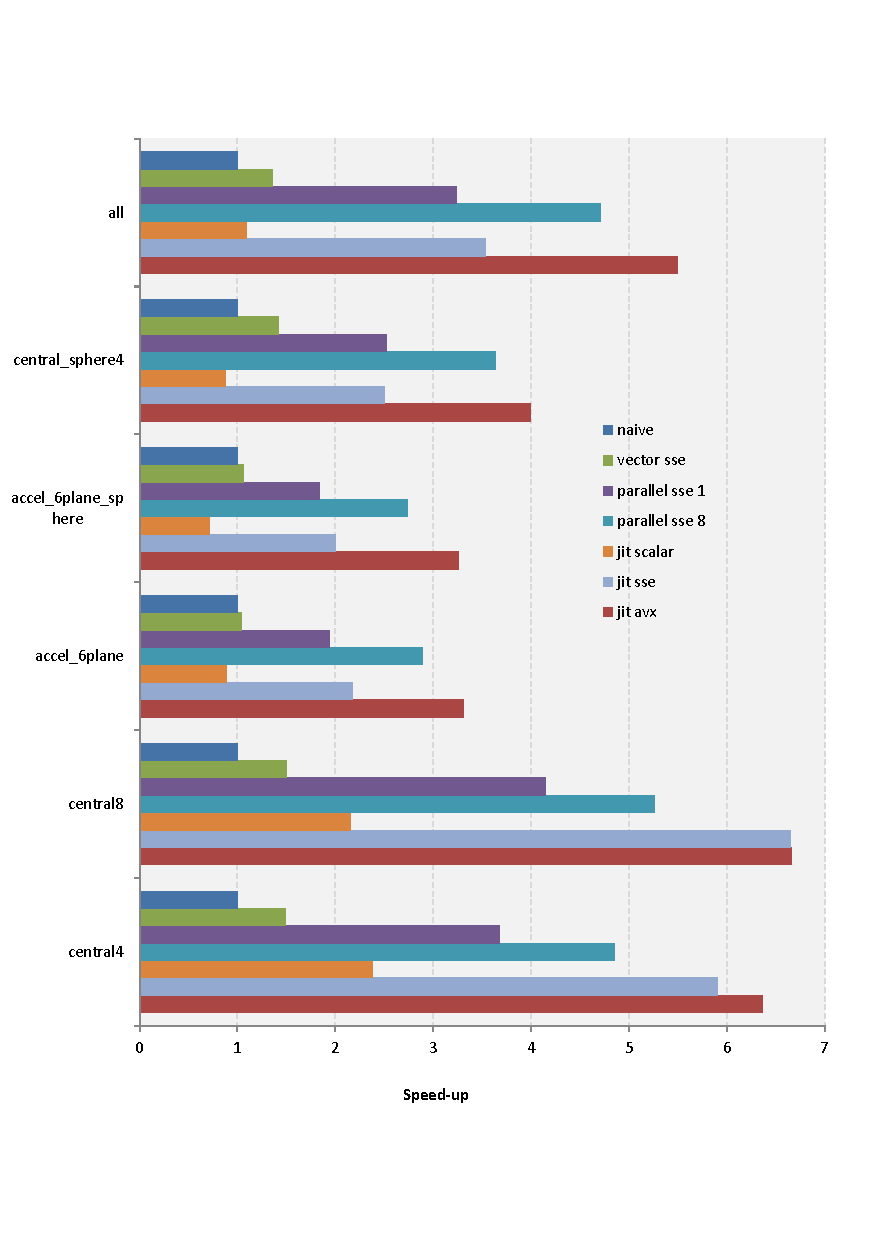
\includegraphics[scale=0.6]{multi_rules.pdf}
  \caption{Performance comparison for multi rule scenarios
  \label{perf_multi}}
\end{figure}

The test cases shown in figure \ref{perf_multi} use more rules at once and we see the results shift in favour of both optimization paths, with an advantage for out JIT compiler. For both the JIT compiled and conventional code the presence of many rules and therefore operations allows to mask the required data shuffling we have seen in the previous comparison. Looking closely at the results we can see that the \texttt{jit avx} code always outperforms every other version, and the \texttt{jit sse} code outperfoming the equivalent hand optimized code, \texttt{parallel sse 1}, as well. Comparing the two conventionally optimized code versions \texttt{parallel sse 1} and \texttt{parallel sse 8} it is clear that the further loop unrolling done in the later is worth the effort, even if the instructions present in the multiple rules all but exhaust the instruction buffers on the cpu and such further unrolling does not provide obvious advantages.

One of the main advantages of the JIT compiler is that it significantly reduces the amount of actually generated instructions. The optimization passes eliminate up to half of the instructions present in the input rules. Due to the types of optimizations that are performed it does however not reduce the critical path length. So the total latency of one loop iteration assuming perfect instruction level paralellism is unaffected. This reinforces the observation that loop unrolling could provide a speed up for the JIT compiled code by allowing more efficient interleaving of independent paths of execution.





\section{Conclusions}

In this paper we have introduced the idea of using a Just In Time compiler for creating simulations of dynamic particle systems. We have then outlined how such a purpose built JIT compiler can take advantage of implicit knowledge and simplified programming requirements. Furthermore we have shown that even a simple implementation can already produce code that is performing at least equivalently or better than conventionally optimized code. Besides direct advantages in performance, having such a JIT compiler also relieves the programmer from having to hand optimize every new simulation rule he might come up with. After the initial effort to create such a JIT compiler its usage provides the best bang for buck for the programmer, he gets the performance of heavily optimized code at the cost of a simple and straight forward implementation. Originally both the conventional code and the JIT compiler were producing SSE code using 128bit wide register with the difference that the JIT compiler only needed little work and changes in the backend to produce new AVX code, while it would be necessary to go over all existing code and redo all the work for the conventional code. This further highlights the advantages of building such an infrastructure, not only to gain immediate performance gains, but also savings for future adjustments when they come along.

Despite the limited scope of this short semester project, we managed to show the value and possible gains of a domain specific JIT compiler, by implementing just a small subset of the tools a conventional compiler uses. In a larger context this also furthers the view that automatic code generation and optimization are worth the effort.

\mypar{Future Work} 
We have already highlighted the possibility of further loop unrolling which allowed the conventional code to partially close the gap to our JIT compiled code. Other possible optimizations not currently implemented include performing algebraic simplifications on the IR and substituting expensive operations such as square roots with fast reverse square root and newton approximations. Another interesting aspect of the online code generation is the possibility to instrument code at runtime and refine heavily used kernels by performing essentially profile guided optimizations for the specific machine the code is currently running on.


%\input{6_Var.tex}


% References should be produced using the bibtex program from suitable
% BiBTeX files (here: bibl_conf). The IEEEbib.bst bibliography
% style file from IEEE produces unsorted bibliography list.
% -------------------------------------------------------------------------
\bibliographystyle{IEEEbib}
\bibliography{bibl_conf}

\end{document}

